\pagebreak
\subsection{Quadratic Probing and Linear Searching Algorithm}
\begin{itemize}
	\item \textbf{Theoretical Time Complexity:}
	      \begin{itemize}
		      \item The time complexity of searching using Quadratic Probing is \(O(n)\).
		      \item The time complexity of searching using Linear Searching Algorithm is \(O(n)\).
	      \end{itemize}
	\item \textbf{Actual execution time:}
	      \begin{itemize}
		      \item Searching using Quadratic Probing is faster than using Linear Searching Algorithm in most cases (except there are too many collisions).
	      \end{itemize}
	\item \textbf{Case Screenshots:}
	      \begin{figure}[!ht]
		      \centering
		      \begin{subfigure}{0.45\textwidth}
			      \centering
			      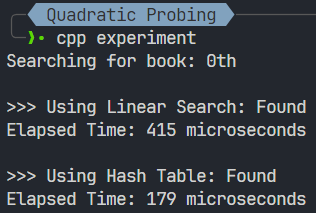
\includegraphics[width=\textwidth]{imgs/Quadratic Probing/beg.png}
			      \caption{When the key is at the begining of Hash Table}\label{fig:quadprobing-beg-metric}
		      \end{subfigure}
		      \hfill
		      \begin{subfigure}{0.45\textwidth}
			      \centering
			      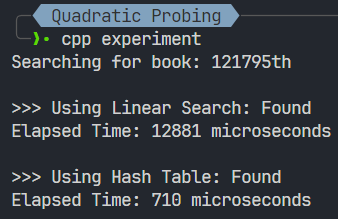
\includegraphics[width=\textwidth]{imgs/Quadratic Probing/mid.png}
			      \caption{When the key is at the middle of Hash Table}\label{fig:quadprobing-mid-metric}
		      \end{subfigure}
		      \hfill
		      \begin{subfigure}{0.45\textwidth}
			      \centering
			      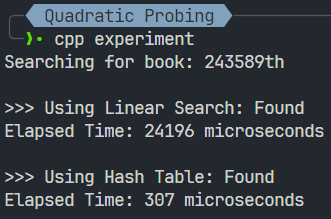
\includegraphics[width=\textwidth]{imgs/Quadratic Probing/end.png}
			      \caption{When the key is at the end of Hash Table}\label{fig:quadprobing-end-metric}
		      \end{subfigure}
		      \hfill
		      \begin{subfigure}{0.45\textwidth}
			      \centering
			      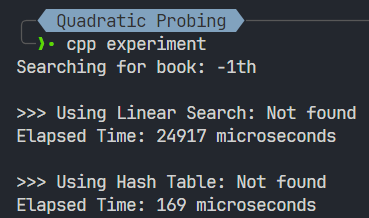
\includegraphics[width=\textwidth]{imgs/Quadratic Probing/not-found.png}
			      \caption{When the key is `not'~in Hash Table}\label{fig:quadprobing-notfound-metric}
		      \end{subfigure}

		      \caption{Screenshots of Searching Case with Quadratic Probing.}\label{fig:quadprobing-search-metric}
	      \end{figure}
\end{itemize}